\documentclass[a4paper, 12pt]{report}
\usepackage[left=1.5in, right=1.0in, top=1.0in, bottom=1.25in]{geometry}
\usepackage{ifpdf}
\usepackage[nocompress]{cite}
\usepackage[pdftex]{graphicx}
\usepackage{balance}
\usepackage{array}
\usepackage{url}
\usepackage{verbatim}
\usepackage{tabularx}
\usepackage{setspace}
\usepackage{comment}
\usepackage{amsmath}
\usepackage{syntax}
\onehalfspacing
\begin{document}
\title{Gorilla v.2: A Compiler for Generating Data-stream Accelerators}
\author{Maysam Lavasani}         
\date{Jun 11, 2014}    % type date between braces
\maketitle

\renewcommand{\thesection}{\arabic{section}}
\small
\setcounter{tocdepth}{4}
\tableofcontents
\normalsize

\section{Introduction}
Gorilla is a compiler for generating high performance 
accelerators that receive incoming streams of data, 
process them, and generate outgoing streams of data. 
The first version of Gorilla was developed as part of the 
research in~\cite{GorillaFPGA2012}. We enhanced Gorilla 
features and developed Gorilla v.2 as part of  
``programmable accelerators'' project. This document 
covers the language specification of Gorilla and, 
also, elaborates on Gorilla hardware compilation process. 

A Gorilla accelerator consists of one or more
processing engine(s) which correspond to different 
stage(s) of processing a data-element in the incoming 
streams of data (See section ~\ref{sec:caseStudy} for 
an example). Each engine is programmed in a stylized-C 
language which gives the impression of sequential 
programming to the designer. Gorilla compiler generates 
a synthesizable hardware model from the engine code. It 
can implement two different concurrency 
mechanisms, pipelining and multi-treading, in the engine 
micro-architecture. The concurrency mechanisms improve 
the quality of the generated accelerator.

%\chapter{Engine language/compiler}
\section{Improvements from Gorilla v.1}
The main improvements in Gorilla v.2 comparing to the 
first version is due to the change of generated output 
language. Gorilla v.1 translates the input program  into 
Verilog code. Gorilla v.2, however, translates the input 
program into Chisel~\cite{ChiselDAC2012}. Chisel is a 
hardware construction language with both object-oriented 
and functional features. The generated Chisel code, later, 
can be fed to the Chisel compiler that can, in turn, 
generates either a synthesizable Verilog model or a 
cycle-accurate C-simulation model.

The new features in Gorilla v.2 include: 
\begin{itemize}
\item Cycle-accurate C-simulation, inherited 
from Chisel C-simulation
\item Support of bundle types, inherited from Chisel 
bundles (see section\ref{sec:dataTypes}) 
\item Split-phase pipelining (see section
~\ref{sec:splitPhasePipelining}) 
\item Support of composing Gorilla engines using 
Chisel code 
\end{itemize}

\section{Gorilla language}
The language for programming an engine is to model a 
state machine consisting of several processing steps 
\footnote{The states in the modeled state machine in
the input program are different from actual hardware 
states. Each state in the input program may be 
translated into one or two hardware state(s) or one 
or two hardware pipeline stages (See section
~\ref{sec:engineCompiler}). To avoid confusion,  
we refer to the states in the input state machine 
as processing steps}.
The input to the Gorilla compiler can be generated by 
a high-level synthesis (HLS) tool from standard C
~\footnote{Currently, gorilla is not integrated with 
any HLS tool. However, our initial study indicates that 
the output of LegUp~\cite{LegUpFPGA2012} scheduler is 
close to Gorilla input language}.  
Alternatively, when the quality of scheduling is critical 
for achieving a high performance, the application can be 
scheduled manually and written directly in form of 
Gorilla input language.

In this section, we use a layer-3 header processor as a 
case study to describe the Gorilla language. We, also, 
discuss individual features and present the Backus-Naur 
Form (BNF) of Gorilla language.  

\subsection{Case study: A layer-3 header processor}
\label{sec:caseStudy}
Figure ~\ref{fig:packetForwardingChain} shows a packet 
processor accelerator which (i) receives an stream of 
incoming packets, (ii) determines the packets destination 
ports based on the result of lookup process, and (iii) 
sends the outgoing packets to the output ports. 

The accelerator consists of five main engines chained 
in a back-to-back fashion. The first engine splits 
the header and payload of the packet, sends the header 
to the output, and stores the payload in a payload 
memory. The second engine assigns a sequencing tag to 
each header. The third engine processes the header and 
determines its destination address. The fourth engine 
reorders the headers based on their sequencing tag. 
This is necessary if the header processor works on 
multiple headers in parallel and cause the headers 
to get out of their incoming order. The last engine 
reassembles the packet from its header and the payload 
that. Lookup and QoS counting engines are used by header 
processor as specialized functional units.

We focus on programming one of the engines in this 
architecture, the header processor. Figure
~\ref{fig:packetProcessingChart} shows the high-level 
flow-chart of the packet processing engine. 
After checking layer-2 and layer-3 headers, the destination 
port is looked up. The engine updates QoS counters 
to keep track of routed packets to a particular destination 
port. Finally, the engine updates the TTL field in the 
packet and, also, updates the checksum field accordingly.
If there is an error in any of these processing steps, the 
packet is marked as an exceptional packet and sent to the 
control-plane~\footnote{In high-end Internet routers network 
processors are part of the router data-plane. The 
control-plane, however, in most cases depends on 
general-purpose hardware. One of the duties of the 
control-plane is handling exceptional packets} 
for further processing.
\begin{figure}
\begin{center}
  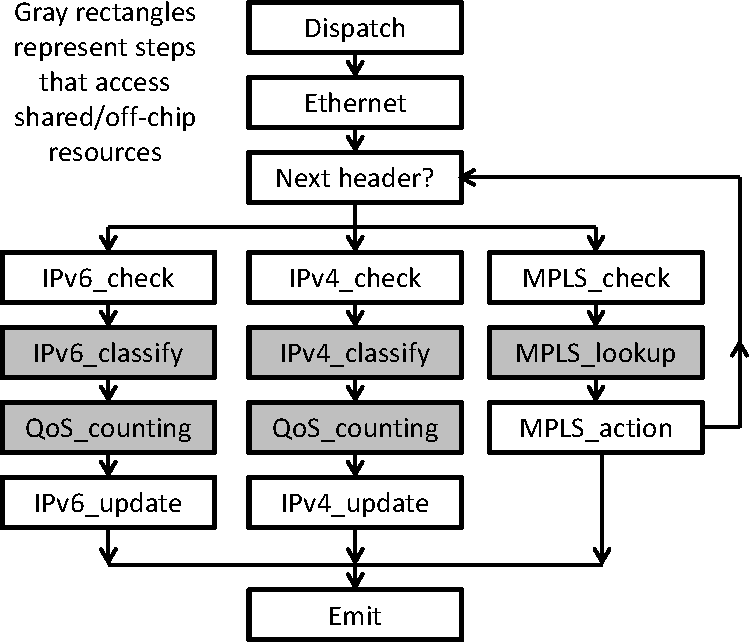
\includegraphics[width = 10cm]{./figures/packetProcessingChart.pdf}
  \caption{IPv4 header processing flow-chart}
  \label{fig:packetProcessingChart}
\end{center}
\end{figure}

\begin{figure}
\begin{center}
  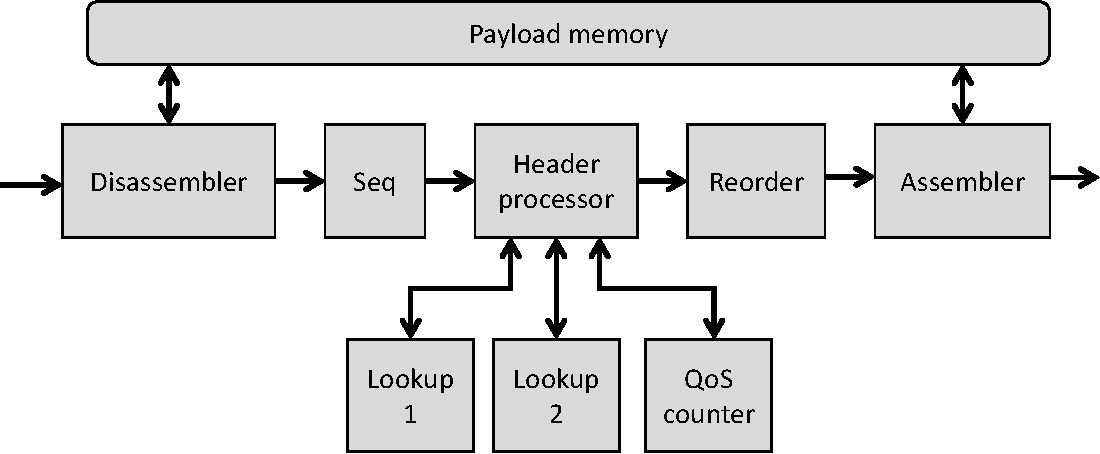
\includegraphics[width = 10cm]{./figures/NPCGPipeline.pdf}
  \caption{A multi-engine accelerator for routing the packets. 
Each engine is generated using Gorilla compiler.}
  \label{fig:packetForwardingChain}
\end{center}
\end{figure}

Following is the gorilla code for implementing the above 
discussed header processor engine. For the sake of 
simplicity, only the code associated with 
processing an IPv4 packet is shown.

\footnotesize
\begin{verbatim}
#pragma INPUT NP_EthMpl3Header_t 
#pragma OUTPUT NP_EthMpl3Header_t 
#pragma OFFLOAD(ipv4Lookup1, uint32_t, uint8_t)
#pragma OFFLOAD(ipv4Lookup2, uint32_t, uint8_t)
#pragma OFFLOAD(qosCount, uint32_t, uint8_t)
#pragma CONCURRENT_SAFE 

typedef struct {
  uint4_t version, hLength;
  uint8_t tos;
  uint16_t length, identification, flagsOffset;
  uint8_t ttl, protocol;
  uint16_t chksum;
  uint32_t srcAddr, dstAddr;
} IPv4Header_t;
typedef struct {
  uint48_t dstAddr, srcAddr;
  uint8_t l3Type, length;
} EthernetHeader_t;
typedef uint1024_t mpl3Header_t;
typedef struct {
 uint8_t outPort;
 EthernetHeader_t  eth;
 mpl3Header_t  l3;
} NP_EthMpl3Header_t;
IPv4Header_t ipv4Input, ipv4Output;
uint32_t gOutPort; 

GS_ETHERNET()
{
  ipv4Input = (IPv4Header_t) Input.l3;
  Output = Input;
  if (Input.l2Protocol == ETHERNET) {
    State = GS_IPV4;
  } else { 
    State = GS_EXCEPTION;
  }
}
GS_IPV4_CHECK()
{
  if (Input.eth.l3Type == IPV4) {
    State = GS_LOOKUP;
    ipv4Output = ipv4Input;
  } else { 
    State = GS_EXCEPTION;
  }
  if (ipv4Input.length < 20 || ipv4Input.version != 4) {
    State = GS_EXCEPTION;
  }
}
GS_IPV4_CLASSIFY()
{
  uint outPort, srcLookupResult;
  outPort = ipv4Lookup1(ipv4Input.dstAddr);
  srcLookupResult = ipv4Lookup2(ipv4Input.srcAddr);
  Output.outPort = outPort;
  gOutPort = outPort;
  if (srcLookupResult == INVALID_ADDRESS || 
   outPort == INVALID_ADDRESS) {
    State = GS_EXCEPTION;
  } else {  
    State = GS_UPDATE;
  }
}
GS_QOS_COUNTING() 
{
  uint8_t qcOutput;
  qcOutput = qosCount(gOutPort);
}
GS_IPv4_UPDATE()
{
  if (ipv4Input.ttl == 1) {
    State = GS_EXCEPTION;
  } else {
    ipv4Output.ttl = ipv4Input.ttl - 1; 
    ipv4Output.chksum = ipv4Input.chksum + 0x80; 
  }
  Output.l3 = (mpl3Header_t) ipv4Output;
  finish();
}
GS_EXCEPTION() 
{
  Output.outPort = CONTROL_PLANE;
  finish();
}
\end{verbatim}
\normalsize


\subsection{Interface specification}
Each engine has one input, one output, and a set of 
offload interfaces. The input and output are one-way 
interfaces. Offloads are two-way interfaces for 
sending requests and receiving the responses.  
The engine interface types are specified using C 
pragmas at the beginning of an engine code. 

Both input and output interfaces of the header 
processing engine are defined as a bundled 
type which consists of Ethernet header and a 
generic type for a layer-3 header. The bundle, 
also, consists of an output port to specify the 
result of lookup process~\footnote{
The output port field in the input interface is 
not used. The same type is used for the input as 
the output for the sake of simplicity}.  

The header processor have three offload interfaces, 
two for connecting to lookup engines and one for 
connecting to QoS counter engine. The pragma for 
defining an offload interface consists of three 
arguments. The Offload name, the input type, and the 
output type. For all of these three offload interfaces, 
the input types are 32 bits and the output types are 
eight bits.
 
\subsection{Processing steps}
Each processing step is defined using a C function 
and can perform arbitrary arithmetic/logic computation. 
The step also can call special purpose functional units. 
The calls are, later, translated to request/response 
messages to/from the functional units through the engine's 
offload interfaces. Each step, also, explicitly specifies 
the next state(s) based on the result of computation and/or 
the responses form functional units. Note that the functional 
units, themselves, are processing engines and can be generated 
by Gorilla compiler.

The packet processing engine consists of six processing 
steps. The lookup processing step calls two lookup functional 
units in parallel. The QoS counting processing step calls the 
QoS counter functional unit.  

\subsection{Data types}
\label{sec:dataTypes}
Apart from standard C data types, Gorilla supports bit accurate 
data types. The bit accurate data types can be specified in forms 
of predefined {\emph uint} data types. For example, {\emph uint48\_t} 
specifies a 48 bits unsigned integer.

Bundled types are specified using C structures. Gorilla translates 
C structures to Chisel bundles. The support of bundled data types 
is specially useful for processing protocol fields and complex data 
structures. The header processor code uses bundled types for 
specifying Ethernet and IPv4 protocols.  

Type casting can be used to convert a variable with 
a given data type to another data type.
Casting a bundle type to another results into 
flattening the source bundle into a bit stream and 
remapping the bit stream into the target bundle type.
The header processor code uses type casting to convert 
a generic layer three header to an IPv4 header bundle.
The programmer, later, can access the IPv4 protocol 
fields as fields of a C structure.
 
\subsection{Predication}
The programmer can use conditional statements in 
each processing step. The conditional statements 
are translated into predication logic by the compiler.
The header processor, for example, uses if-statements 
to check whether there is an error in processing the 
header.

\subsection{Transitioning between processing steps}
Transitioning between processing steps are done 
by explicit assignments to {\bf State} variable.
At the end of each processing step, the Gorilla 
infrastructure switches to the processing step that 
is specified by this variable.

\subsection{Input/output operations}
The input data element is accessible through   
{\bf Input} variable. Output should be assigned 
to {\bf Output} variable. 
Receiving an input is done implicitly when engine 
restarts in the first processing step. Sending an 
output is done either by calling {\bf finish} 
routine or {\bf emit} routine. The difference 
between finish and emit is that finish returns 
to the first processing step of the engine but 
emit returns back to the processing step specified 
as its argument.  
By calling the finish method, the header processor 
emits the output header and also returns back to the 
first processing step.

\subsection{Engine language BNF}
\begin{grammar}
<program> ::= <interface-pragmas> <type-defintions> 
<variable-defintions> <processing-steps> 
\alt <type-defintions>

<interface-definitions> ::= <input-defintion> 
<output-defintion> <offload-defintions>

<input-definition> ::= `#pragma' `INPUT' `(' 
<type-ident> `)'

<output-definition> ::= `#pragma' `OUTPUT' `(' 
<type-ident> `)'

<offload-defintions> ::= <offload-definition> 
<offload-definitions>
\alt <offload-definition>

<offload-definition> ::= `#pragma` `OFFLOAD' `(' 
<type-identifer> `,' <offload-ident> `)'

<variable-defintions> ::= <variable-definition> 
<variable-definitions>
\alt <variable-definitions>

<variable-definition> ::= <type-ident> <variable-list>

<varialbe-list> ::= <variable-id> <variable-list>
\alt <variable-id>

<processing-steps> ::= <processing-step> 
\alt <processing-step> <processing-steps>

<statatement-list> ::= <statement> <statement-list> 
\alt <statement> 

<processing-step> ::= <processing-step-name> `( )' `{' 
<variable-defintions> <statment-list> 
<offload-statement-list> <statement-list> `}'

<statement> ::= <ident> `=' <expr> `;' 
\alt <if-else-statement>
\alt <if-statement>
\alt `{' <stattement-list> `}' 
\alt <emit-statement> 

<if-statement> ::= `if' `(' <expr> `)' `{' 
<statement-list> `}'   

<if-else-statemnt> ::= if-statement `else` `{' 
<statement-list> `}'

<offload-statement-list> ::= <offload-statement> 
<offload-statement-list> 
\alt <offload-statement>

<expr> ::= <ident> <binary-operator> <expr>
\alt <ident>
\alt <cast-prefix> <expr> 
\alt <ident> <field-expression>

<cast-prefix> ::= `(' <type-identifier> ')'

<field-expression> ::= `.' <ident> 
\alt `.' <ident> <field-expression>

<offload-statement> ::= <ident> `=` <offload-ident> `(' 
<expr> `)' `;'

<emit-statement> ::= `finish' `(' `)' `;'
\alt `emit' `(' <processing-step-name> `)' `;'

<type-definitions> ::= <type-defintion> 
<type-defintions>
\alt <type-defintion>

<type-defintion> ::= `typedef' <type-id-new> 
<type-id-old>
\alt `typedef' `struct' `{' <variable-defnitions> `}' 
<bundle-type-id> `;'

\end{grammar}

\section{Engine execution model}
This section covers communication mechanism, the type of 
parallelism, and the support for global state in Gorilla. 
These concepts form the underlying execution model for 
Gorilla engines. 
  
\subsection{Latency-insensitive interfaces}
\label{sec:latencyInsensitive}
Gorilla engines use latency-insensitive protocol
~\cite{theoryOfLatencyInsenssitiveDesigns} for 
communicating through input, output, and offload 
interfaces. For each way of an interface a valid 
signal from the source to the sink indicates whether 
the source has a data element to transfer. Also, a 
ready signal from the sink to the source indicates 
whether the sink is ready to receive a data 
element. Transfer happens when both of these signals 
are asserted.

\subsection{Global state memory}
Gorilla engines cannot keep any internal data that is 
accessible by processing steps associated with two 
different input data-elements. Therefore, if we reset all 
engine's registers after processing a data-element, 
the outcome of the computation  will be the same
~\footnote{We are assuming 
that the engine has single thread. If it has more than 
one thread after a thread finishes processing a data-element,  
resetting that particular thread's registers will not affect 
the outcome of the computation}.

Gorilla engines can keep the global state, between 
processing of data-elements, in offloaded memory 
elements, however. The QoS counter in header processor 
example is a global state that is accessible by 
processing steps of all headers.

\subsection{Data-parallel execution}
We assume that there is no dependency 
between processing steps. As the result, 
the generated concurrency mechanisms in 
the hardware, either multi-threading or 
pipelining, does not preserve any dependency 
between processing steps of different 
input data-elements. 

If any dependency exists between processing 
the input data-elements, the programmer (or the 
front-end compiler) should use synchronization 
mechanisms as offloaded functional units to enforce 
the priority in scheduling the threads or stalling 
the pipeline.

\section{Engine templates}
\label{sec:engineCompiler}
Gorilla compiler uses a template-based method 
to compiler processing steps into the hardware.
Templates are generic and highly parametrized 
form of the hardware that will be specialized 
based on the functionality specified in the input 
program. The template is designed for arbitrary 
number of functional units, arbitrary number of 
processing steps, and arbitrary data types for 
interfaces. 

Gorilla has three main templates that generate 
(i) simple state machine engines, (ii) multi-threaded 
engines, and (iii) pipelined engines.

\subsection{Simple state machine engines}
\begin{figure}
\begin{center}
  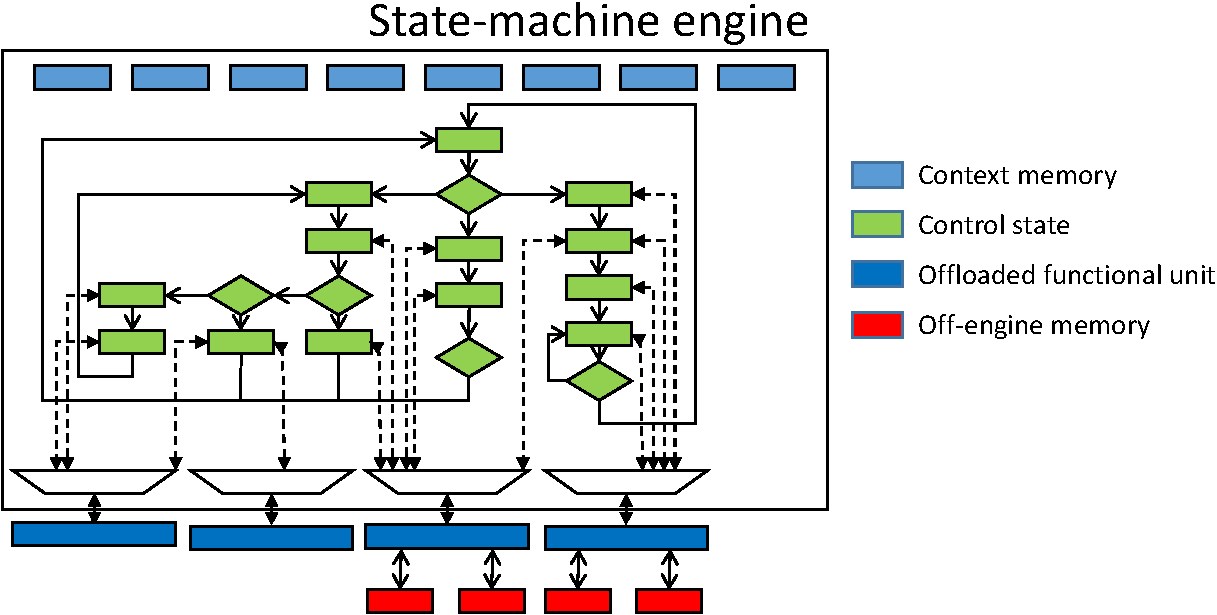
\includegraphics[width = 14cm]{./figures/engineTemplates/FSMEngineTemplate.pdf}
  \caption{A simple state machine engine with}
  \label{fig:FSMtemplate}
\end{center}
\end{figure}
When an engine is translated into a single state machine 
all processing steps that do not have any offload calls 
are translated into a single hardware state and all processing 
steps that have offload calls are translated into two hardware 
states, a state for computations before offload call(s), preOff 
state, and a state for computations after offload call(s), 
postOff state. Global variables are translated into registers 
and local variables are translated into wires. Figure~\ref{fig:FSMtemplate} 
shows an implemented engine using a simple state machine template.



\subsection{Multi-threaded engines}
\begin{figure}
\begin{center}
  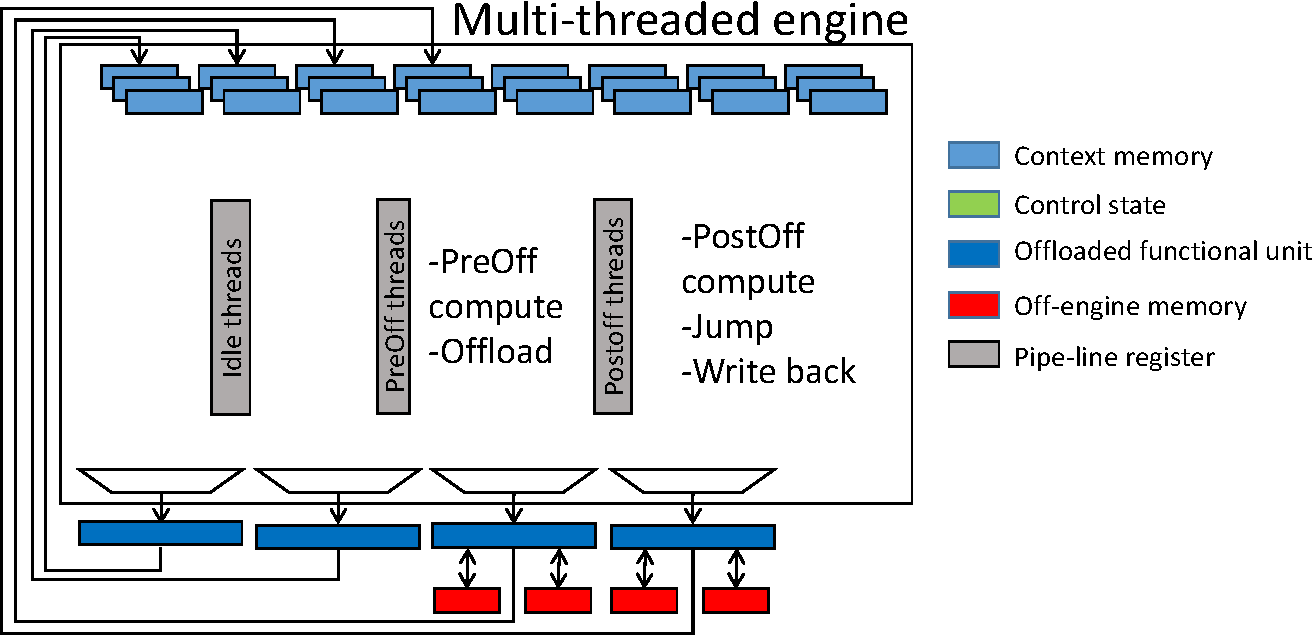
\includegraphics[width = 12cm]{./figures/engineTemplates/MTEngineTemplate.pdf}
  \caption{A multi-threaded engine}
  \label{fig:MTTemplate}
\end{center}
\end{figure}
Since the target applications of Gorilla are data-parallel 
in nature, whenever an engine is spending a large amount 
of time in the offload call(s), it is reasonable to switch 
to the processing of another input data element while 
waiting for the response of the offload call(s). Inspired by 
multi-threading technique in high-performance processors
~\cite{SMT}, we refer to this type of concurrency 
as multi-threading. Each thread in an engine is responsible 
for processing an input data-element. Whenever a thread 
calls an offload, the engine switches to another thread, 
processing another input data-element. Therefore, offload 
latencies in a thread are hidden by performing computation in 
other threads. 
 
\subsubsection{Execution pipeline}
A multi-threaded engine (shown in Figure~\ref{fig:MTTemplate}) 
executes the processing steps using a two-stage execution 
pipeline. The first stage of the pipeline, also known as preOff 
stage, executes all the computations of a processing step 
before the offload calls. The second stage, also known as 
postOff stage, executes the computations after offload calls. 
The thread associated to a given data-element is either in 
preOff stage or postOff stage of the execution pipeline. 
Therefore, the preOff and postOff computations of a single 
input data element are not executed at the same clock cycle. 
Therefore, RAW, WAW, or WAR dependencies cannot occur for a 
single thread. 

The engine keeps track of threads using three bit-vectors. 
The first bit-vector indicates whether a thread is idle and 
waiting for an input data-element. The second bit-vector 
contains all threads that are in preOff stage, either 
performing the preOff computations or waiting for offload 
request acknowledgement. The third bit-vector contains all 
threads that are in postOff stage, either performing the 
postOff computations or waiting for offload replies. 
 

\subsubsection{Thread contexts}
Thread contexts consist of all global variables in the 
input engine program. It, also, includes the implicit 
variables including Input, Output, State, and emitReturnState 
(See section \ref{sec:rcvSend}) variables. Each of these 
variables is stored in a register array which is indexed using 
thread id of the current active thread.  

\subsubsection{Receive/send processing steps}
\label{sec:rcvSend}
Each thread in a processing engine has an invisible 
processing step for receiving an input data-element. 
Also, it has an invisible processing step for sending 
an output data-element.

The free threads stays in receive processing step 
until an input data-element is assigned to them.
When a new data-element arrives, a thread from the 
pool of available threads is selected and assigned 
for processing the data-element. The State variable 
for the thread is changed to the first processing 
step in the Gorilla program. The engine assert the 
ready signal on its input as long as there is an 
available free thread in the engine.
  
When threads emit an output, they automatically switch 
to the send processing step. An implicit variable keeps 
track of the step that the thread should switch to after 
successfully sending the output element. A thread stays 
in the send processing step until it receives the assertion 
of transfer (on the ready signal of the output port). While 
staying in this processing step, the engine asserts its valid 
signal on the output port.
 
\subsubsection{Offload dispatch and wakeup logic}
Apart from the preOff computations specified in a 
processing step, the preOff stage is responsible 
for generating request(s) to offloaded functional units. 
The engine leaves the preOff stage and enters the postOff 
stage whenever all requests for all offload calls in a 
particular processing step are accepted by the 
corresponding functional units.  Also, the engine leaves 
the postOff stage and enter the preOff stage of the next 
processing step whenever all replies form the offload calls 
are received~\footnote{It is possible that more than one 
thread becomes available to move from postOff stage to preOff stage. 
A fair arbiter selects one of these threads at any given cycle.}. 

When a thread in a preOff stage calls an offloaded functional 
unit, a request is sent to the functional unit by asserting 
the valid signal on the corresponding request port. 
The request is kept asserted until the functional unit acknowledge 
receiving the request by asserting the ready signal on the same 
port (See Figure~\ref{fig:offloadDispatchLogic} for 
details). The actual request data that is the argument of 
the offload call is derived along the request valid signal 
(Offload request bus is not shown in the Figure).
The dispatch logic for a given functional unit can be 
asserted by any of the processing steps that call the 
functional unit.  
When last response from functional units of a given 
processing step receives, the corresponding thread is 
waken up and moved from postOff thread list to preOff 
thread list for processing the next Gorilla processing 
step . Figure~\label{fig:offloadThreadWakeupLogic} shows 
the logic that determines if a given thread is done waiting 
for its offload calls in postOff stage. 
 
\begin{figure}
\begin{center}
  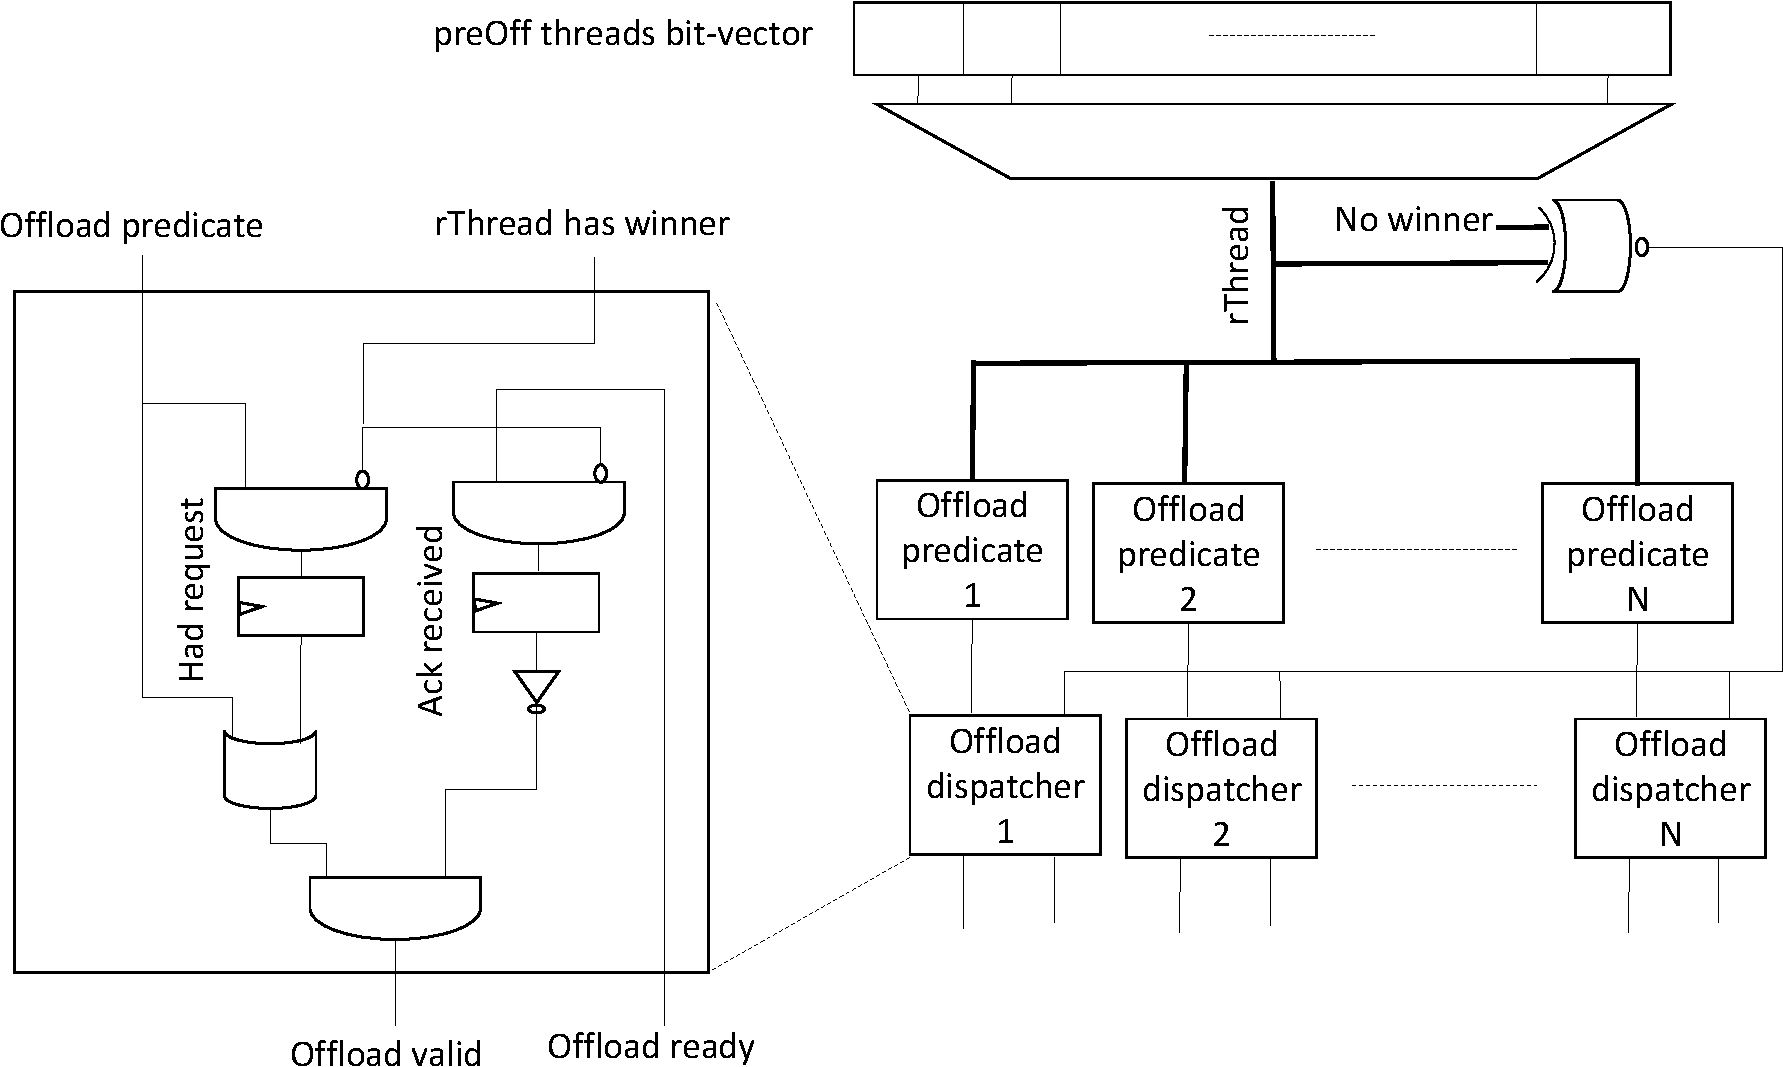
\includegraphics[width = 12cm]{./figures/offloadDispatchLogic.pdf}
  \caption{Offload dispatch logic}
  \label{fig:offloadDispatchLogic}
\end{center}
\end{figure}

\begin{figure}
\begin{center}
  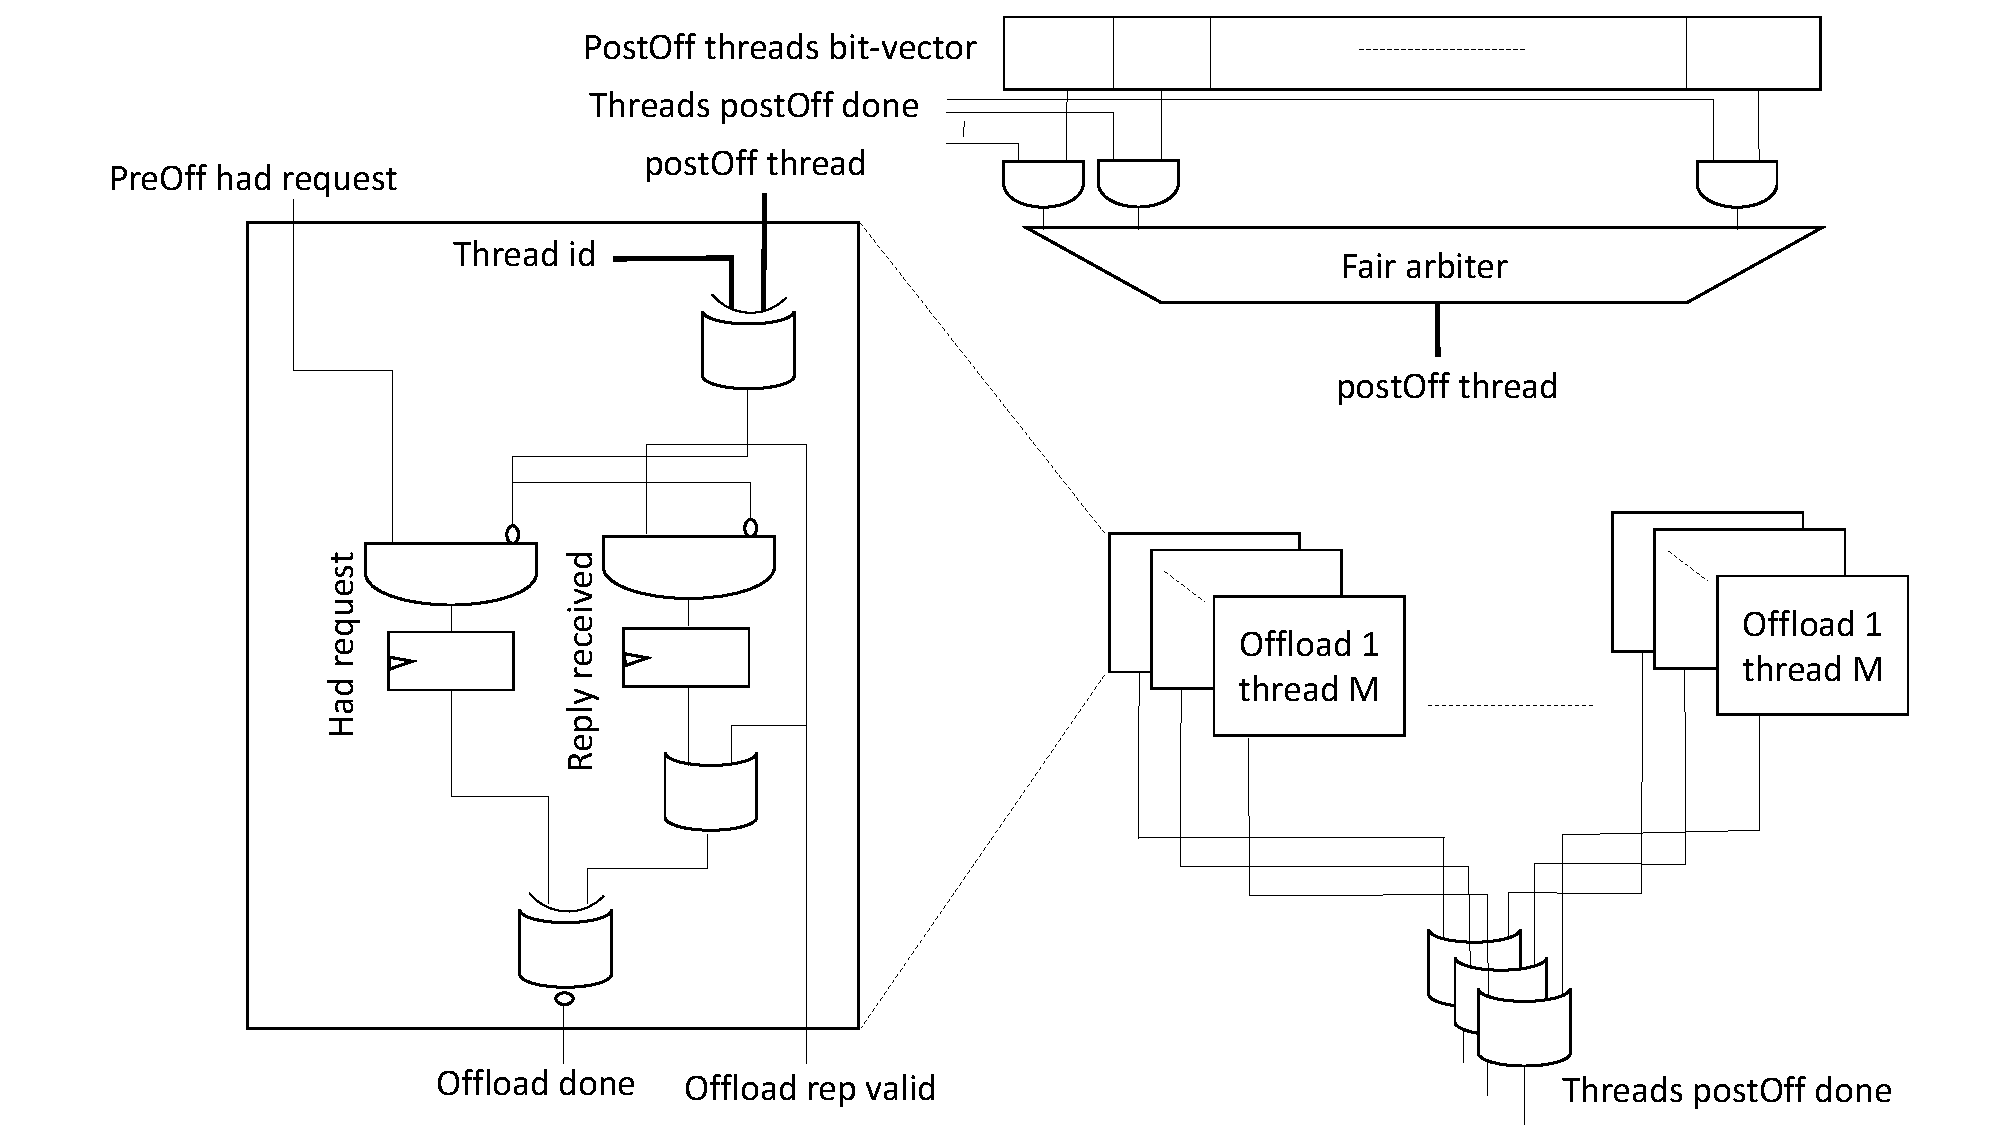
\includegraphics[width = 12cm]{./figures/offloadThreadWakeupLogic.pdf}
  \caption{Offload thread wakeup logic}
  \label{fig:offloadThreadWakeupLogic}
\end{center}
\end{figure}


\subsection{Pipelined engines}
Whenever the control flow between processing steps is 
solely jump from one state to its next step (in the input 
program order), Gorilla can generate a pipelined engine.

Pipelining improves the throughput of an engine and 
can be useful if computation in the engine is a bottleneck 
in the design (multi-threading is useful when stalling on 
the offloaded functional units is a bottleneck in the design).

\begin{figure}
\begin{center}
  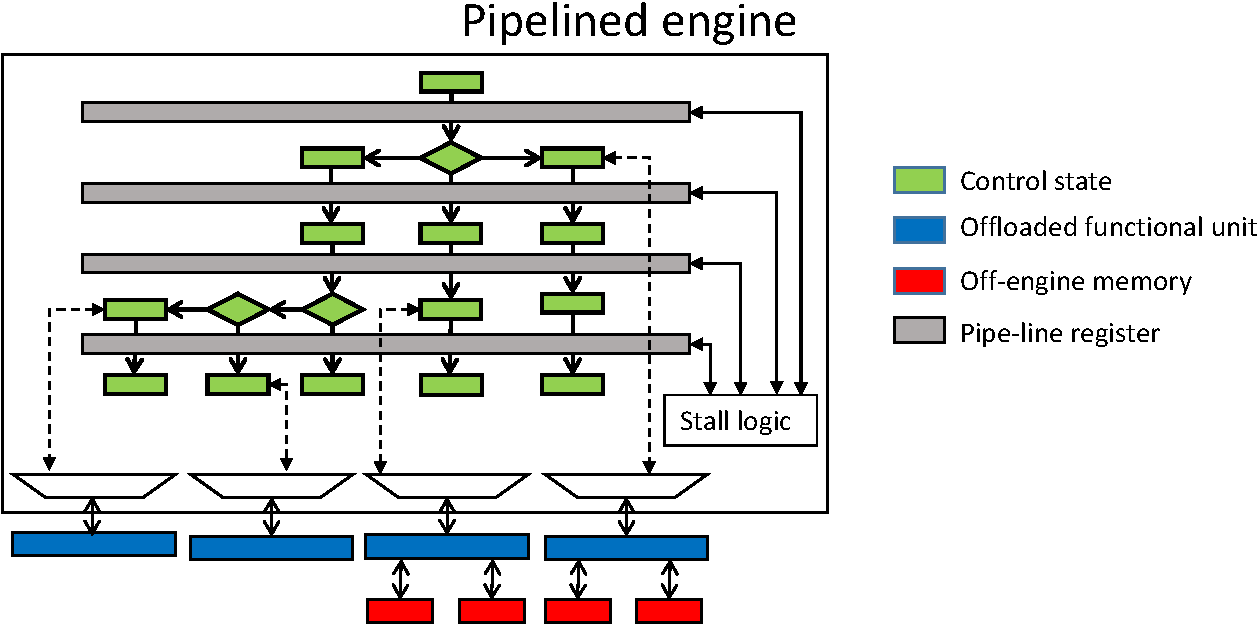
\includegraphics[width = 12cm]{./figures/engineTemplates/PipelinedEngineTemplate.pdf}
  \caption{A pipeline engine for a loop-free input Gorilla program}
  \label{fig: Pipelined template}
\end{center}
\end{figure}
\subsubsection{Pipeline registers}
Pipelined engine does not have any global context. 
The global variables are kept in pipeline registers.
For a given input data element, corresponding global 
variables are marching along the input data element 
through the pipeline stages.

\subsubsection{Receive/send stages}
A dedicated receive stage is added at the start of each 
Gorilla pipeline and a dedicated send stage is added at the 
end of each Gorilla pipeline.

\subsubsection{Split-phase stages}
\label{sec:splitPhasePipelining}
Unlike other pipelining HLS tools, Gorilla code can call 
offload functional units and wait for the response of 
functional units without stalling the whole pipeline.
Gorilla compiler generates a preOff pipeline stage and a 
postOff pipeline stage for every processing step with a 
call to offloaded functional unit.

The structure of preOff dispatch logic and postOff wakeup 
logic in a pipelined engine is similar to the corresponding 
stages in a multi-threaded engine. The main difference, however, 
is that unlike multi-threaded engine which uses the same execution 
pipeline for all processing steps, a pipelined engine has dedicated 
preOff and postOff stages for each processing step 
with offload calls. 

\subsubsection{Stall logic}
In a pipelined engine, in addition to engine interfaces
each pipeline stage follows the latency-insensitive 
protocol (Described in~\ref{sec:latencyInsensitive}). 
A preOff stage is stalled when there is not postOff thread 
available for accepting the result of preOff stage. When a 
preOff stage is stalled it ripple back the stall by 
de-asserting the ready signal. A postOff stage is stalled, 
however, whenever its next stage is stalled.
The ready signal of the receive pipeline stage is connected to the 
whole engine ready signal and the valid signal of the send pipeline 
stage is connected to the whole engine valid signal.

\section{Conclusion}
This document described the details on the language 
specification and the hardware generation process 
of Gorilla compiler. Our preliminary experience 
with Gorilla show that high quality hardware can 
be generated by combining engines that are generated 
by Gorilla. The concurrency mechanisms which are 
automatically generated by Gorilla is essential 
in the quality of generated hardware. The combination 
of one-way input/output and two-way offload interfaces 
provide an expressive way to describe various compositions 
of interacting engines. 
%\chapter{Composition language/compiler}
%\section{Composition language}
%\subsection{Motivation example: a network processor}
%\subsection{Composition language BNF}
\bibliographystyle{plain}
\bibliography{./bib}

\end{document}

